\documentclass[10pt]{article}
\usepackage[a4paper, margin=2cm]{geometry}
\usepackage[utf8]{inputenc}
\usepackage{graphicx}
\usepackage{lastpage}
\usepackage{fancyhdr}
\usepackage{tikz}
\usetikzlibrary{trees}
\pagestyle{fancy}
\fancyhf{}
\rfoot{Page \thepage \hspace{1pt} sur \pageref{LastPage}}

\begin{document}

\title{Math : Probabilités - Partie II}
\author{Hovinne Noé}
\date{24.05.20}
\maketitle
\vspace{1cm}
\subsection*{Exercice 1.3}
Un étudiant estime que la probabilité qu'il réussisse son examen d'anglais est 0,7 ; qu'il réussisse son examen de français de 0,6 et la probabilité qu'il réussisse les deux examens est de 0,4.\vspace{6pt}

Calcule la probabilité que l'étudiant :\vspace{2pt}

\hspace{10pt}a) réussisse en anglais, sachant qu'il a réussi en français.\vspace{1pt}

\hspace{10pt}b) échoue en anglais, sachant qu'il a réussi en français.\vspace{1pt}

\hspace{10pt}c) échoue en anglais, sachant qu'il a échoué en français.\vspace{12pt}

a) Posons les événements $A$ "Réussite en anglais" et $B$ "Réussite en français" :

$$P(A\mid B)=\frac{P(A\cap B)}{P(B)}=\frac{0,4}{0,6}=\frac{2}{3}$$\vspace{1pt}

b) Posons les événements $C$ "Échec en anglais" et $B$ "Réussite en français" :

$$P(C\mid B)=\frac{P(C\cap B)}{P(B)}=\frac{0,2}{0,6}=\frac{1}{3}$$\vspace{1pt}

c) Posons les événements $C$ "Échec en anglais" et $D$ "Échec en français" :

$$P(C\mid D)=\frac{P(C\cap D)}{P(D)}=\frac{0,1}{0,4}=\frac{1}{4}$$

\subsection*{Exercice 11, page 298}
Donner une estimation de la probabilité d'avoir "421" lorsqu'on lance trois dés.\vspace{6pt}

Il y a 6 combinaisons qui nous intéressent: 421, 412, 241, 214, 142, 124 sur les $6^3$ combinaisons possibles.

On réalise donc le calcul suivant afin de déterminer la probabilité de l'événement $A$ "avoir 4, 2 et 1" :

$$P(A)=\frac{6}{216}=\frac{1}{36}\approx 0.0277777$$\vspace{1pt}

En lançant les trois dés, nous avons approximativement 2,77\% de chances de former le nombre 421.

En exécutant 1000 lancés des trois dés, nous pouvons poser à postériori que nous formerons 28 fois le nombre 

421.
\newpage

\subsection*{Exercice 12, page 299}
Dans un restaurant, 60\% des menus proposent de la viande, 30\% des menus proposent de la glace et 20\% des menus ne proposent ni viande ni glace.\vspace{6pt}

a) Présentation des données dans un tableau à double entré :

\begin{center}
\begin{tabular}{ |c|c|c|c| } 
 \hline
 & \textbf{Avec Viande} & \textbf{Sans Viande} & \textbf{Total} \\ 
 \hline
 \textbf{Avec Glace} & 10\% & 20\% & 30\%\\ 
 \hline
 \textbf{Sans Glace} & 50\% & 20\% & 70\%\\ 
 \hline
 \textbf{Total} & 60\% & 40\% & 100\%\\
 \hline
\end{tabular}
\end{center}

b) On considère les événements V "le menu comprend de la viande" et G "le menu comprend de la glace".\vspace{6pt}

\hspace{10pt}1) $P(V)=0,6$\vspace{4pt}

\hspace{10pt}2) $P(V\cap G)=0,1$\vspace{4pt}

\hspace{10pt}3) $P(V\cap \bar{G})=0,5$\vspace{4pt}

\hspace{10pt}4) $P(V\cup G)=0,8$\vspace{4pt}\vspace{6pt}

c) $(V\cap \bar{G})$ et $(\bar{V} \cap G)$ ne sont pas compatibles parce que l'intersection de ces deux ensembles est nulle. 

\hspace{12pt}De plus, étant donné qu'un ensemble est composé d'un événement et que l'autre est composé de son 

\hspace{12pt}complémentaire dans  $\Omega$, il est impossible que ces ensembles soient compatibles.

\subsection*{Exercice 13, page 299}
\subsubsection*{a. On tire successivement et \textit{avec remise} 3 boules d'une urne contenant 6 boules vertes et 4 boules jaunes.}

\hspace{16pt}1) Calcul de la probabilité du tirage successif de 3 boules de même couleur :\vspace{1cm}


% Set the overall layout of the tree
\tikzstyle{level 1}=[level distance=3.5cm, sibling distance=3.5cm]
\tikzstyle{level 2}=[level distance=3.5cm, sibling distance=2cm]
\tikzstyle{level 3}=[level distance=3.5cm, sibling distance=1cm]

% Define styles for bags and leafs
\tikzstyle{bag} = [text width=4em, text centered]
\tikzstyle{end} = [circle, minimum width=3pt,fill, inner sep=0pt]

% The sloped option gives rotated edge labels. Personally
% I find sloped labels a bit difficult to read. Remove the sloped options
% to get horizontal labels. 
\begin{tikzpicture}[grow=right, sloped]
\node[bag] {}
    child {
        node[bag] {\textbf{Jaune}}        
            child {
                node[bag] {\textbf{Jaune}}
                    	child {
            			node[bag] {\textbf{Jaune}}
                		edge from parent
                		node[above] {}
                		node[below]  {$\frac{4}{10}$}
            			}
            			child {
            			node[bag] {Verte}
                		edge from parent
                		node[above] {$\frac{6}{10}$}
                		node[below]  {}
            			}
                edge from parent
                node[above] {}
                node[below]  {$\frac{4}{10}$}
            }
            child {
                node[bag] {Verte}
                edge from parent
                node[above] {$\frac{6}{10}$}
                node[below]  {}
            }
            edge from parent 
            node[above] {}
            node[below]  {$\frac{4}{10}$}
    }
    child {
        node[bag] {\textbf{Verte}}        
        child {
                node[bag] {Jaune}
                edge from parent
                node[above] {}
                node[below]  {$\frac{4}{10}$}
            }
            child {
                node[bag] {\textbf{Verte}}
                    child {
            			node[bag] {Jaune}
                		edge from parent
                		node[above] {}
                		node[below]  {$\frac{4}{10}$}
            			}
            			child {
            			node[bag] {\textbf{Verte}}
                		edge from parent
                		node[above] {$\frac{6}{10}$}
                		node[below]  {}
            			}
                edge from parent
                node[above] {$\frac{6}{10}$}
                node[below]  {}
            }
        edge from parent         
            node[above] {$\frac{6}{10}$}
            node[below]  {}
    };
\end{tikzpicture}\vspace{1cm}

\hspace{13pt}La probabilité du tirage successif de 3 boules de même couleur est égale à :

$$ \left( \frac{6}{10} \right) ^3+ \left( \frac{4}{10} \right) ^3=\frac{216}{1000}+\frac{64}{1000}=0,216+0,064=21,6\%+6,4\%=28\%$$\vspace{0,1cm}

\newpage

\hspace{2pt}2) Calcul de la probabilité du tirage successif de 2 boules vertes et d'une boule jaune :\vspace{1cm}

% Set the overall layout of the tree
\tikzstyle{level 1}=[level distance=3.5cm, sibling distance=3.5cm]
\tikzstyle{level 2}=[level distance=3.5cm, sibling distance=2cm]
\tikzstyle{level 3}=[level distance=3.5cm, sibling distance=1cm]

% Define styles for bags and leafs
\tikzstyle{bag} = [text width=4em, text centered]
\tikzstyle{end} = [circle, minimum width=3pt,fill, inner sep=0pt]

% The sloped option gives rotated edge labels. Personally
% I find sloped labels a bit difficult to read. Remove the sloped options
% to get horizontal labels. 
\begin{tikzpicture}[grow=right, sloped]
\node[bag] {}
    child {
        node[bag] {Jaune}        
            child {
                node[bag] {Jaune}
                    	child {
            			node[bag] {Jaune}
                		edge from parent
                		node[above] {}
                		node[below]  {$\frac{4}{10}$}
            			}
            			child {
            			node[bag] {Verte}
                		edge from parent
                		node[above] {$\frac{6}{10}$}
                		node[below]  {}
            			}
                edge from parent
                node[above] {}
                node[below]  {$\frac{4}{10}$}
            }
            child {
                node[bag] {Verte}
                edge from parent
                node[above] {$\frac{6}{10}$}
                node[below]  {}
            }
            edge from parent 
            node[above] {}
            node[below]  {$\frac{4}{10}$}
    }
    child {
        node[bag] {\textbf{Verte}}        
        child {
                node[bag] {Jaune}
                edge from parent
                node[above] {}
                node[below]  {$\frac{4}{10}$}
            }
            child {
                node[bag] {\textbf{Verte}}
                    child {
            			node[bag] {\textbf{Jaune}}
                		edge from parent
                		node[above] {}
                		node[below]  {$\frac{4}{10}$}
            			}
            			child {
            			node[bag] {Verte}
                		edge from parent
                		node[above] {$\frac{6}{10}$}
                		node[below]  {}
            			}
                edge from parent
                node[above] {$\frac{6}{10}$}
                node[below]  {}
            }
        edge from parent         
            node[above] {$\frac{6}{10}$}
            node[below]  {}
    };
\end{tikzpicture}\vspace{1cm}

\hspace{13pt}La probabilité du tirage successif de 2 vertes et d'une boule jaune est égale à :

$$\frac{6}{10}\times \frac{6}{10}\times \frac{4}{10}=\frac{18}{125}=0,144=14,4\%$$\vspace{0,1cm}

\subsubsection*{b. On tire successivement et \textit{sans remise} 3 boules d'une urne contenant 6 boules vertes et 4 boules jaunes.}

\hspace{16pt}1) Calcul de la probabilité du tirage successif de 3 boules de même couleur :\vspace{1cm}

% Set the overall layout of the tree
\tikzstyle{level 1}=[level distance=3.5cm, sibling distance=3.5cm]
\tikzstyle{level 2}=[level distance=3.5cm, sibling distance=2cm]
\tikzstyle{level 3}=[level distance=3.5cm, sibling distance=1cm]

% Define styles for bags and leafs
\tikzstyle{bag} = [text width=4em, text centered]
\tikzstyle{end} = [circle, minimum width=3pt,fill, inner sep=0pt]

% The sloped option gives rotated edge labels. Personally
% I find sloped labels a bit difficult to read. Remove the sloped options
% to get horizontal labels. 
\begin{tikzpicture}[grow=right, sloped]
\node[bag] {}
    child {
        node[bag] {\textbf{Jaune}}
            child {
                node[bag] {\textbf{Jaune}}
                    	child {
            			node[bag] {\textbf{Jaune}}
                		edge from parent
                		node[above] {}
                		node[below]  {$\frac{2}{8}$}
            			}
            			child {
            			node[bag] {Verte}
                		edge from parent
                		node[above] {$\frac{6}{8}$}
                		node[below]  {}
            			}
                edge from parent
                node[above] {}
                node[below]  {$\frac{3}{9}$}
            }
            child {
                node[bag] {Verte}
                edge from parent
                node[above] {$\frac{6}{9}$}
                node[below]  {}
            }
            edge from parent 
            node[above] {}
            node[below]  {$\frac{4}{10}$}
    }
    child {
        node[bag] {\textbf{Verte}}
        child {
                node[bag] {Jaune}
                edge from parent
                node[above] {}
                node[below]  {$\frac{4}{9}$}
            }
            child {
                node[bag] {\textbf{Verte}}
                    child {
            			node[bag] {Jaune}
                		edge from parent
                		node[above] {}
                		node[below]  {$\frac{4}{8}$}
            			}
            			child {
            			node[bag] {\textbf{Verte}}
                		edge from parent
                		node[above] {$\frac{4}{8}$}
                		node[below]  {}
            			}
                edge from parent
                node[above] {$\frac{5}{9}$}
                node[below]  {}
            }
        edge from parent         
            node[above] {$\frac{6}{10}$}
            node[below]  {}
    };
\end{tikzpicture}\vspace{1cm}

\hspace{13pt}La probabilité du tirage successif de 3 boules de même couleur est égale à :

$$\left[ \frac{6}{10} \times \frac{5}{9} \times \frac{4}{8}\right] + \left[ \frac{4}{10} \times \frac{3}{9} \times \frac{2}{8} \right]=0,2=20\%$$\vspace{0,1cm}

\hspace{2pt}2) Calcul de la probabilité du tirage successif de 2 boules vertes et d'une boule jaune :\vspace{1cm}

\tikzstyle{level 1}=[level distance=3.5cm, sibling distance=3.5cm]
\tikzstyle{level 2}=[level distance=3.5cm, sibling distance=2cm]
\tikzstyle{level 3}=[level distance=3.5cm, sibling distance=1cm]

\tikzstyle{bag} = [text width=4em, text centered]
\tikzstyle{end} = [circle, minimum width=3pt,fill, inner sep=0pt]

\begin{tikzpicture}[grow=right, sloped]
\node[bag] {}
    child {
        node[bag] {Jaune}
            child {
                node[bag] {Jaune}
                    	child {
            			node[bag] {Jaune}
                		edge from parent
                		node[above] {}
                		node[below]  {$\frac{2}{8}$}
            			}
            			child {
            			node[bag] {Verte}
                		edge from parent
                		node[above] {$\frac{6}{8}$}
                		node[below]  {}
            			}
                edge from parent
                node[above] {}
                node[below]  {$\frac{3}{9}$}
            }
            child {
                node[bag] {Verte}
                edge from parent
                node[above] {$\frac{6}{9}$}
                node[below]  {}
            }
            edge from parent 
            node[above] {}
            node[below]  {$\frac{4}{10}$}
    }
    child {
        node[bag] {\textbf{Verte}}
        child {
                node[bag] {Jaune}
                edge from parent
                node[above] {}
                node[below]  {$\frac{4}{9}$}
            }
            child {
                node[bag] {\textbf{Verte}}
                    child {
            			node[bag] {\textbf{Jaune}}
                		edge from parent
                		node[above] {}
                		node[below]  {$\frac{4}{8}$}
            			}
            			child {
            			node[bag] {Verte}
                		edge from parent
                		node[above] {$\frac{4}{8}$}
                		node[below]  {}
            			}
                edge from parent
                node[above] {$\frac{5}{9}$}
                node[below]  {}
            }
        edge from parent         
            node[above] {$\frac{6}{10}$}
            node[below]  {}
    };
\end{tikzpicture}\vspace{1cm}

\hspace{13pt}La probabilité du tirage successif de 2 vertes et d'une boule jaune est égale à :

$$\frac{6}{10}\times \frac{5}{9}\times \frac{4}{8}=\frac{1}{6}\approx 0,1666\approx 16,66\%$$\vspace{0,1cm}


\subsection*{Exercice 14, page 299}
Un camp de vacances héberge 80 personnes ; 55 d'entre elles pratiquent la natation, 33 vacanciers dont 16 nageurs jouent au tennis.\vspace{2pt}

Calcul de la probabilité qu'une personne choisir au hasard ne pratique ni le tennis ni la natation :

\begin{center}
\begin{tabular}{ |c|c|c|c| } 
 \hline
 & \textbf{Pratique la natation} & \textbf{Ne pratique pas la natation} & \textbf{Total} \\ 
 \hline
 \textbf{Pratique le tennis} & 16 & 17 & 33\\
 \hline
 \textbf{Ne pratique pas le tennis} & 39 & \textbf{8} & 47\\ 
 \hline
 \textbf{Total} & 55 & 25 & 80\\
 \hline
\end{tabular}
\end{center}

\hspace{13pt}La probabilité qu'une personne choisie au hasard ne pratique ni le tennis ni la natation est égale à :
$$\frac{8}{80}=0,1=10\%$$

\subsection*{Exercice 16, page 300}
\subsubsection*{a. Un dé est truqué de telle sorte que la probabilité pour que le "1" apparaisse est 1/3 tandis que les autres événements élémentaires sont équiprobables.}

\hspace{15pt}1) Calcul de la probabilité d'apparition de "2" :

$$\frac{2}{3} \times \frac{1}{5}=\frac{2}{15}\approx 0,1333 \approx 13,33\%$$

2) Calcul de la probabilité que "2" n'apparaisse pas :

$$1- \frac{2}{15} = \frac{13}{15}\approx 0,8666 \approx 86,66\%$$

3) Calcul de la probabilité d'obtenir un nombre pair :

$$\frac{2}{15}+\frac{2}{15}+\frac{2}{15}=\frac{6}{15}=0,4=40\%$$

\newpage

4) Calcul de la probabilité d'obtenir un nombre impair :

$$\frac{1}{3}+\frac{2}{15}+\frac{2}{15}=0,6=60\%$$

\subsubsection*{b. On truque un dé de telle sorte que les résultats pairs aient des chances égales d'apparaître et les résultats impairs aient aussi la même chance d'apparaître. Mais on s'arrange pour que chaque résultat pair ait deux fois plus de chances d'apparaître que n'importe quel résultat impair.}

Calcul de la probabilité d'obtenir un résultat impair/pair :\vspace{2pt}

\hspace{13pt}Étant donné que le nombre de résultats pairs et impairs est le même, et que la probabilité d'obtenir un 

\hspace{13pt}nombre pair est deux fois plus grande que la probabilité d'obtenir un nombre impair,

\hspace{13pt}on répartit les probabilités comme suit :

\begin{center}$P($résultat pair$\displaystyle )=\frac{2}{3}$ et $P$(résultat impair)$\displaystyle =\frac{1}{3}$\end{center}
\subsection*{Exercice 17, page 300}
Dans un lavoir un lavoir industriel, un jour donné, chaque lessiveuse est susceptible de subir deux types de panne : l'une d'origine électronique avec une probabilité de 0,002 ($P(E)=0,002$) et l'autre, mécanique, avec une probabilité de 0,006 ($P(M)=0,006$).\vspace{2pt}

a. Calcul de la probabilité que $L_1$ ait les deux types de panne le même jour :

$$P(E)\times P(M)=0,002\times 0,006=0,000012=0,0012\%$$\vspace{1pt}

b. Calcul de la probabilité que $L_2$ n'ait aucune panne le même jour :

$$1-P(M\cup E)=1-\left[ P(M)+P(E)-P(M\cap E) \right]=1-0,007788=0,992012=99,2012\%$$\vspace{1pt}

c. Calcul de la probabilité que $L_1$ et $L_2$ soient toutes les deux en panne le même jour :

$$[P(M\cup E)]^2=(0,007988)^2=0,000063808144=0,0063808144\%$$

\subsection*{Exercice 19, page 301}
Deux étudiants doivent résoudre un problème sans se consulter. Ils peuvent trouver la solution avec des probabilités respectivement égales à 0,7 et 0,4. Quelle est la probabilité que le problème ne soit pas résolu ?

$$1-P(A\cup B)=1- \left[ P(A)+P(B)-\left( P(A)\times P(B)\right)\right]=1-[0,7+0,4-0,28]=1-0,82=0,18=18\%$$

\subsection*{Exercice 20, page 301}
On tire une carte au hasard d'un jeu de 52 cartes. On considère les événements suivants :\vspace{2pt}

$A$ "tirer une carte rouge" ;

$B$ "tirer une dame" ;

$C$ "tirer une carte de pique" ;

$D$ "tirer une figure (valet - dame - roi)".

\subsubsection*{a. Calcul de la probabilité de chacun de ces événements :}

$$P(A)=\frac{26}{52}=0,5=50\%$$

$$P(B)=\frac{4}{52}=\frac{1}{13}\approx 0,07692307692O\approx 7,69\%$$

$$P(C)=\frac{13}{52}=0,25=25\%$$

$$P(D)=\frac{12}{52}\approx 0,2307692308\approx 23,08\%$$

\newpage

\subsubsection*{b. Signification des événements suivants :}

\hspace{15pt}$A\cap D=$ "tirer une carte rouge qui a une figure".

$B\cup C=$ "tirer une dame ou une carte de pique".

$B\mid C=$ "tirer une dame" sachant que l'on a déjà tiré l'ensemble des cartes de pique.

$D\mid A=$ "tirer une figure" sachant que l'on a déjà tiré l'ensemble des cartes rouges.

\subsubsection*{c. Vérification de l'indépendance des événements $B$ et $C$ :}

\hspace{15pt}Par définition, deux événements sont indépendants si la réalisation de l'un ne modifie pas la probabilité 

de l'autre. 

Dans cet exercice, $P(B\mid C)=P(B)$ car $\displaystyle P(B\mid C)=\frac{P(B\cap C)}{P(C)}=\frac{1}{13}$

Et $P(C\mid B)=P(C)$ car $\displaystyle P(C\mid B)=\frac{P(C\cap B)}{P(B)}=\frac{1}{4}$\vspace{4pt}

Les événements $B$ et $C$ sont donc indépendants l'un de l'autre.



\subsection*{Exercice 21, page 301}
Soient $A$ et $B$ des événements indépendants tels que $\displaystyle P(A)=\frac{1}{2}$ et $\displaystyle P(A\cup B)=\frac{2}{3}$.

$$P(B)=P(A\cup B)-P(A)+P(A\cap B)$$

$$P(B)=\frac{2}{3}-\frac{1}{2}+\frac{P(B)}{2}$$

$$P(B)=2\times \frac{1}{6}=\frac{1}{3}$$

$$P(A\mid B)=P(A)=\frac{1}{2}$$

$$P(B\mid A)=P(B)=\frac{1}{3}$$
\subsection*{Exercice 22, page 301 et 302}
L'histogramme (\textit{fig. 22}) donne la répartition des salaires mensuels en euros dans une entreprise.

\subsubsection*{a. On interroge une personne au hasard.}

\hspace{16pt}1) La probabilité que son salaire soit supérieur à 2400 euros est égale à :

$$\frac{30}{150}=20\%$$

2) La probabilité qu'elle gagne moins de 2000 euros est égale à :

$$\frac{82}{150}\approx 54,67\%$$

\subsubsection*{b. On interroge une personne qui gagne plus de 2400 euros.}

\hspace{16pt}1) La probabilité qu'elle gagne plus de 3200 euros est égale à :

$$\frac{5}{30}\approx 16,67\%$$

2) La probabilité qu'elle gagne au moins 2800 euros est égale à :

$$\frac{14}{30}\approx 46,67\%$$

\newpage

\subsection*{Exercice 24, page 303}
\subsubsection*{a. On lance deux fois successivement un dé tétraédrique bien équilibré et on s'intéresse à la somme des points obtenus.}

\begin{figure}[h]
    \textit{\caption{Représentation de la fréquence d'apparition de la somme des résultats obtenus}}\vspace{6pt}
    \centering
    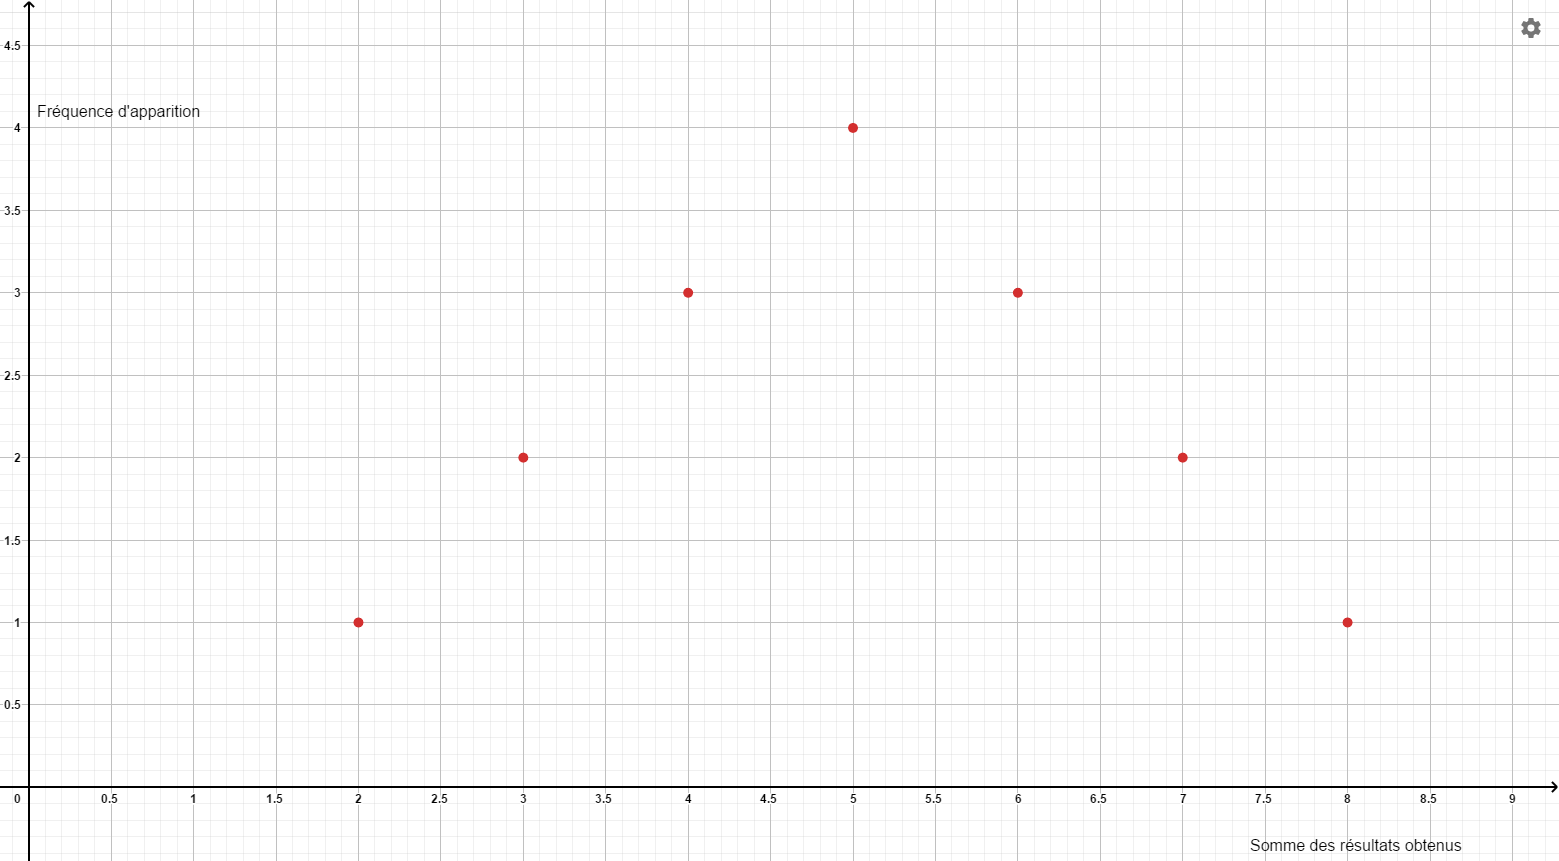
\includegraphics[width=12cm, height=5.5cm]{assets/Exercice 24a.png}
\end{figure}

Détermination de la probabilité de l'événement $A$ "obtenir un résultat inférieur ou égal à 4" :

$$P(A)=\frac{6}{16}=37,5\%$$

\subsubsection*{b. On lance deux dés cubiques, de couleurs différentes, bien équilibrés.}

\hspace{15pt}1) La probabilité que la somme des résultats soit de 7 est égale à :

$$\frac{6}{36}\approx 16,67\%$$

2) La probabilité que la somme des résultats soit de 9 est égale à :

$$\frac{4}{36}\approx 11,11\%$$

3) La probabilité que la somme des résultats soit inférieure ou égale à 6 est égale à :

$$\frac{15}{36}\approx 41,67\%$$

4) La probabilité que la somme des résultats soit de 7 ou 11 est égale à :

$$\frac{8}{36}\approx 22,22\%$$

5) La probabilité que les dés aient des résultats identiques est égale à :

$$\frac{6}{36}\approx 16,67\%$$

6) La probabilité que la différence positive entre les deux résultats soit supérieure ou égale à 3 est égale à :

$$\frac{12}{36}\approx 33,34\%$$

7) La probabilité que la somme des résultats soit inférieure ou égale à 7, sachant qu'au moins un des résultats

\hspace{12pt}est pair est égale à :

$$\frac{15}{36}\approx 41,67\%$$

\begin{center}
\vspace{1cm}Ce travail a été réalisé en \LaTeX . \vspace{0.2cm}

La figure 1 a été construite sur \textit{GeoGebra}.\vspace{0.2cm}
\end{center}

\end{document}
